\section{Поддержка Java-платформы в среде "<MPS">}
Ядро среды "<MPS"> написано на кросс-платформенном языке "<Java"> \cite{eckel}. В связи с этим в среде "<MPS"> существуют развитые средства для взаимодействия с Java-платформой. Для написания Java-кода в среде "<MPS"> разработан язык "<jetbrains.mps.baseLanguage"> (далее "<baseLanguage">). Этот язык является почти полной реализацией спецификации "<Java 5"> \cite{java5spec}. В нем определены такие концепты, как "<класс">, "<интерфейс">, "<метод">, "<предложение">, "<выражение"> и т.д.

Библиотеки, написанные непосредственно на языке "<Java">, могут быть использованы при разработке кода на языке "<baseLanguage">. Для этого среда "<MPS"> предоставляет доступ к пакетам библиотек, как к моделям. Классы, поля и методы из этих пакетов представляются экземплярами соответствующих концептов языка "<baseLanguage">.

Таким образом, для того, чтобы в своей модели написать на языке "<baseLanguage"> класс, выводящий на консоль сообщение "<Hello, world!">, необходимо добавить в набор, используемых моделью языков --- "<baseLanguage">, а в набор, импортированных моделей ---
"<java.lang@java\_stub"> и "<java.io@java\_stub">
(Рис. \ref{fig:Import}). Суффикс "<@java\_stub"> в именах моделей, указывает на то, что эти модели являются на самом деле пакетами языка "<Java">.
\begin{figure}
 \centering
 \fbox{
  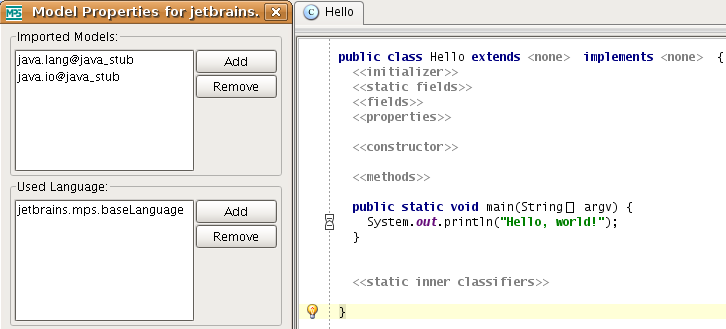
\includegraphics[width=\textwidth]{Import.png}
 }
 \caption{Код класса, выводящего на консоль строку «Hello, world!», и список используемых языков и импортированных моделей}
 \label{fig:Import}
\end{figure}
